\chapter{2023/12/18}\label{20231218}

\section{Vibration of a one-dimensional semi-infinite rod
一维半无限长杆的振动}\label{vibration-of-a-one-dimensional-semi-infinite-rod-ux4e00ux7ef4ux534aux65e0ux9650ux957fux6746ux7684ux632fux52a8}

\begin{center}
    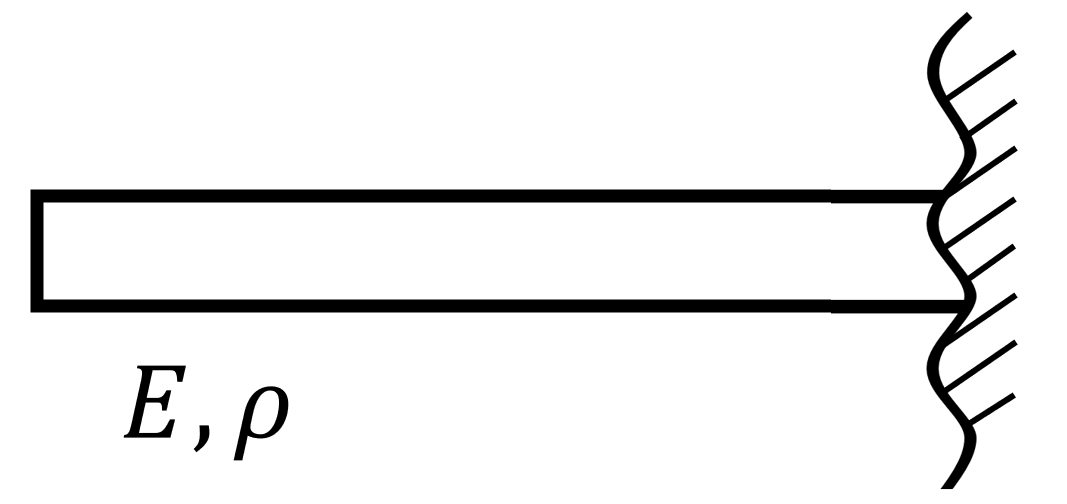
\includegraphics[height=40pt]{assets/One-dimensional_semi-infinite_rod.png}
    \captionof{figure}{One-dimensional semi-infinite rod}
\end{center}

As shown in Fig 27.1, we assume that the rod has density \(\rho\) and Young's modulus
(杨氏模量) \(E\).

\subsection*{(1) Dimensional analysis
量纲分析}\label{dimensional-analysis-ux91cfux7eb2ux5206ux6790}

The dimension of density and Young's modulus are
\[[E] = \frac{[F]}{[A]} = \frac{\mathrm{MLT^{-2}}}{\mathrm{L^2}} = \mathrm{ML^{-1}T^{-2}}\]
and \[[\rho] = \mathrm{ML^{-3}}.\]
\[\left[ \frac{E}{\rho} \right] = \mathrm{L^2 T^{-2}} = [c^2],\] and
thus we know \[c \sim \sqrt{\frac{E}{\rho}}.\]

\subsection*{(2) Lagrangian mechanics
拉格朗日力学}\label{lagrangian-mechanics-ux62c9ux683cux6717ux65e5ux529bux5b66}

The kinetic energy, written as the integral of a segment of the rod from
\(x\) to \(x + \mathrm{d}x\) is
\[T = \int_{0}^{+\infty} \frac{1}{2} \rho A \mathrm{d}x \left( \frac{\partial u}{\partial t} \right)^2,\]
and the potential energy is
\[U = \int_{0}^{+\infty} \frac{1}{2} EA \left( \frac{\partial u}{\partial x} \right)^2 \mathrm{d}x.\]

Write \(L = T - U\) as
\[L = \int_{0}^{+\infty} \mathcal{L} \mathrm{d}x,\] and we have
\[\mathcal{L} = \frac{1}{2} \left[ \rho \left( \frac{\partial u}{\partial t} \right)^2 - E \left( \frac{\partial u}{\partial x} \right)^2 \right]A.\]

According to the expanded Euler-Lagrangian equations, putting \(x\) and
\(t\) in the same position, we know
\[\frac{\partial}{\partial t} \frac{\partial \mathcal{L}}{\partial (\partial u / \partial t)} + \frac{\partial}{\partial x} \frac{\partial \mathcal{L}}{\partial (\partial u / \partial x)} - \frac{\partial \mathcal{L}}{\partial u} = 0,\]
and we get
\[\left( \frac{1}{c^2} \frac{\partial^2}{\partial t^2} - \frac{\partial^2}{\partial x^2} \right) u = \Box u = 0,\]
where \[c = \sqrt{\frac{E}{\rho}}.\]

\section[Deriving Hamilton's canonical equations 推导哈密顿正则方程]{Derivation of Hamilton's canonical equations
哈密顿正则方程的推导}\label{derivation-of-hamiltons-canonical-equations-ux54c8ux5bc6ux987fux6b63ux5219ux65b9ux7a0bux7684ux63a8ux5bfc}

\subsection*{(1) Conjugate variable pairs
共轭变量对}\label{conjugate-variable-pairs-ux5171ux8f6dux53d8ux91cfux5bf9}

\begin{itemize}
\tightlist{}
\item
  Thermodynamics

  In thermodynamics, we have conjugate pairs
  \(\left\{ \begin{array}{l}T \\ S \end{array} \right.\),
  \(\left\{ \begin{array}{l} p \\ V \end{array} \right.\) and
  \(\left\{ \begin{array}{l} \mu \\ N \end{array} \right.\), and
  correspondingly we have the \textbf{fundamental thermodynamic relation
  (热力学基本方程)}:
  \[\mathrm{d}U = T \mathrm{d}S - p \mathrm{d}V + \sum_i \mu_i \mathrm{d}N_i.\]

  \emph{编者注:课上赵老师写的是
  \(\mathrm{d}F = \mathrm{d}U - T \mathrm{d}S + p \mathrm{d}V + \mu \mathrm{d}n\),查询热力学教材、维基百科等资料发现疑似有误。}
\item
  Work conjugate

  In analytical mechanics, we have one famous conjugate pair of force
  and generalized force \[\left\{
        \begin{array}{ll}
            \boldsymbol{F} & \mathrm{d} \boldsymbol{r} \\
            Q & \delta q
        \end{array}
    \right.\] and they have the relation
  \[\sum_{i = 1}^{n} \boldsymbol{F}_i \cdot \delta \boldsymbol{r}_i = \sum_{i = 1}^{n} \boldsymbol{F}_i \cdot \left( \sum_{j = 1}^{s} \frac{\partial \boldsymbol{r}_i}{\partial q_j} \delta q_j \right) = \sum_{j = 1}^{s} \left( \sum_{i = 1}^{n} \boldsymbol{F}_i \cdot \frac{\partial \boldsymbol{r}_i}{\partial q_j} \right) \delta q_j = \sum_{j = 1}^{s} Q_j \delta q_j.\]
\item
  Generalized coordinates conjugate

  \[\left\{
    \begin{array}{ll}
        \displaystyle Q_j = \frac{\partial L}{\partial q_j} \quad \quad & \delta q_j  \\[1.5ex]
        \displaystyle p_j = \frac{\partial L}{\partial \dot{q_j}} & \dot{q_j}
    \end{array}
    \right.\]
\end{itemize}

\subsection*{(2) Advantages and drawbacks of Lagrangian mechanics
拉格朗日力学的优势和缺陷}\label{advantages-and-drawbacks-of-lagrangian-mechanics-ux62c9ux683cux6717ux65e5ux529bux5b66ux7684ux4f18ux52bfux548cux7f3aux9677}

\begin{itemize}
\tightlist{}
\item
  Advantage:

  Newtonian mechanics is a kind of mechanics illustrated graphically,
  while Lagrangian mechanics utilizes the energy method (使用能量方法)
  and stands at a higher level.
\item
  Drawbacks:

  \begin{enumerate}
  \def\labelenumi{\arabic{enumi}.}
  \tightlist{}
  \item
    From
    \(\displaystyle {\partial L \over \partial{q}_j} = {\mathrm{d} \over \mathrm{d}t} {\partial L \over \partial \dot{q}_j}\),
    we can see that \({q}_j\) and \(\dot{q}_j\) are not equal.
  \item
    The dimension system is complicated. For example, if \(q_1\) has a
    length dimension, then \(q_1 \dot{q}_1\) has a dimension of
    \(\mathrm{L^2T^{-1}}\); if \(q_2\) has an angle dimension, then
    \(q_1 \dot{q}_1\) has a dimension of \(\mathrm{T^{-1}}\). These two
    don't match.
  \end{enumerate}

  Hamiltonian mechanics uses \(q_j\) and \(p_j\) as its basic
  coordinates, and we know that \(q_j p_j\) has the dimension of action:
  \[[q_j p_j] = [E] \cdot [t].\]

  \emph{所以说,哈密顿力学比拉格朗日力学更美,是经典力学美的高峰。}
\end{itemize}

\subsection*{(3) Mathematical form of Legendre transformation
勒让德变换的数学形式}\label{mathematical-form-of-legendre-transformation-ux52d2ux8ba9ux5fb7ux53d8ux6362ux7684ux6570ux5b66ux5f62ux5f0f}

Suppose we have a function \(f = f(x, y)\).

Take the total differential of \(f\), and we acquire
\[\mathrm{d}f = \frac{\partial f}{\partial x} \mathrm{d}x + \frac{\partial f}{\partial y} \mathrm{d}y.\]

Here, we let \(\displaystyle u = \frac{\partial f}{\partial x}\) and
\(\displaystyle v = \frac{\partial f}{\partial y}\). Introduce a new
function \(g = ux - f\), and the differential of \(g\) is
\[\mathrm{d}g = u \mathrm{d}x + x \mathrm{d}u - \mathrm{d}f = x \mathrm{d}u - v \mathrm{d}y.\]

\subsection*{(4) Using Legendre transformation to derive the
Hamilton's canonical equations
用勒让德变换推导哈密顿正则方程}\label{using-legendre-transformation-to-derive-the-hamiltons-canonical-equations-ux7528ux52d2ux8ba9ux5fb7ux53d8ux6362ux63a8ux5bfcux54c8ux5bc6ux987fux6b63ux5219ux65b9ux7a0b}

In the derivation above, let \(f\) be the Lagrangian \(L\), \(g\) be the
Hamiltonian \(H\), \(x\) be the generalized velocity \(\dot{q}\) and
\(y\) be the generalized coordinate \(q\). Substitute this in, and we
get \[H = \dot{p} \dot{q} - L.\]

According to this, we can present the \textbf{Legendre transformation
(勒让德变换)} in analytical mechanics. In a system with \(n\) particles
and \(s\) generalized coordinates,
\[H = \sum_{j = 1}^{s} p_j \dot{q}_j - L.\]

Take the differential of both sides ,and we get
\[\mathrm{d}H = \sum_{j = 1}^{s} \left( p_j \mathrm{d} \dot{q}_j + \dot{q}_j \mathrm{d} p_j \right) - \mathrm{d}L. \quad(1)\]

Take the total derivative of \(L = L(q_j, \dot{q}_j, t)\), and we know
that \begin{align*}
    \mathrm{d}L & = \frac{\partial L}{\partial t} \mathrm{d}t + \sum_{j = 1}^{s} \left( \frac{\partial L}{\partial q_j} \mathrm{d}q_j + \frac{\partial L}{\partial \dot{q}_j} \mathrm{d} \dot{q}_j \right) \\
    & = \frac{\partial L}{\partial t} \mathrm{d}t + \sum_{j = 1}^{s} \left( \dot{p}_j \mathrm{d}q_j + {p}_j \mathrm{d} \dot{q}_j \right). \quad(2)
\end{align*}

Substitute \((2)\) into \((1)\), and we get
\[\mathrm{d}H = \sum_{j = 1}^{s} \dot{q}_j \mathrm{d} p_j - \sum_{j = 1}^{s} \dot{p}_j \mathrm{d}q_j - \frac{\partial L}{\partial t} \mathrm{d}t. \quad(3)\]

Also, because \(H = H(q_j, p_j, t)\), take the full derivative of \(H\)
and we get
\[\mathrm{d}H = \frac{\partial H}{\partial t} \mathrm{d}t + \sum_{j = 1}^{s} \left( \frac{\partial H}{\partial q_j} \mathrm{d}q_j + \frac{\partial H}{\partial p_j} \mathrm{d} p_j \right). \quad(4)\]

Compare equations \((3)\) and \((4)\) to observe that \[\left\{
    \begin{aligned}
        \frac{\partial H}{\partial q_j} &= -\dot{p}_j, \\
        \frac{\partial H}{\partial p_j} &= \dot{q}_j,
    \end{aligned}
\right.\] which are the \textbf{Hamiltonian Canonical equations
(哈密顿正则方程)}.

\subsection*{(5) SHO example
以简谐振子为例}\label{sho-example-ux4ee5ux7b80ux8c10ux632fux5b50ux4e3aux4f8b}

Use the displacement from the equilibrium point \(x\) as the generalized
coordinate, and the Hamiltonian and Lagrangian of the SHO are
\[H = \frac{p^2}{2m} + U(x)\] and
\[L = \frac{1}{2} m \dot{x}^2 - \frac{1}{2} kx^2.\]

Using Legendre transformation, we acquire
\[H = p \dot{x} - L = m \dot{x}^2 - \left( \frac{1}{2} m \dot{x}^2 - \frac{1}{2} kx^2 \right) = \frac{1}{2} m \dot{x}^2 + \frac{1}{2} kx^2 = \frac{p^2}{2m} + \frac{1}{2} kx^2.\]

Substitute \(H\) into the Hamiltonian Canonical equations, and we
acquire \[- \dot{p} = \frac{\partial H}{\partial x} = kx\] and
\[\dot{x} = \frac{\partial H}{\partial p} = \frac{p}{m}.\]

Take the time derivative of \(\displaystyle \dot{x} = \frac{p}{m}\),
substitute the result into \(-\dot{p} = kx\), and we get
\[m \ddot{x} = - kx,\] \[\ddot{x} + \frac{k}{m} x = 0,\]
\[\ddot{x} + \omega^2_0 x = 0.\]

Also, we can put the SHO into phase space (相空间) \((x, p)\) and we can
get an ellipse (椭圆). Every dot in the phase space represents a
possible state of the SHO. All the dots in the phase space, i.e.~all
possible states of the SHO, form the ellipse known as the \textbf{phase
trajectory (相轨道)}. The direction of the phase flow (相流) is
clockwise (顺时针).

\begin{center}
    \begin{tikzpicture}[scale=1.5]
        \draw[->] (-2, 0) -- (2,0) node[below] {$x$};
        \draw[->] (0, -2) -- (0,2) node[left] {$p$};
          
        \node at (1.5, 0) [above right] {$\sqrt{2E / k}$};
        \node at (0, 1) [above left] {$\sqrt{2mE}$};
        
        \draw[->] (1.299, -0.5) arc (330:-30:1.5 and 1);
        
        \node at (1.7, 1.3) {Phase trajectory};
        \node at (1.3, -0.5)[below right] {Direction of phase flow};
    \end{tikzpicture}
    \captionof{figure}{Phase space of SHO}
\end{center}

Suppose the initial phase (初相位) of the SHO is \(\varphi_0\), and we know
\[x = \sqrt{\frac{2E}{k}} \cos \left( \sqrt{\frac{k}{m}} t + \varphi_0 \right)\]
and
\[p = - \sqrt{2mE} \sin \left( \sqrt{\frac{k}{m}} t + \varphi_0 \right).\]

\subsection*{(6) The conservation of the Hamiltonian
哈密顿量的守恒}\label{the-conservation-of-the-hamiltonian-ux54c8ux5bc6ux987fux91cfux7684ux5b88ux6052}

When we look again at equations \((3)\) and \((4)\), we can see that
\[- \frac{\partial L}{\partial t} = \frac{\partial H}{\partial t}.\]

When Lagrangian \(L\) does not depend on \(t\),
\(\displaystyle \frac{\partial L}{\partial t} = 0\), and thus
\(\displaystyle \frac{\partial H}{\partial t} = 0\).

Using \((4)\), we can get \begin{align*}
    \frac{\mathrm{d}H}{\mathrm{d}t} & = \frac{\partial H}{\partial t} + \sum_{j = 1}^{s} \left( \frac{\partial H}{\partial q_j} \frac{\mathrm{d}q_j}{\mathrm{d}t} + \frac{\partial H}{\partial p_j} \frac{\mathrm{d} p_j}{\mathrm{d}t} \right) \\
    & = \frac{\partial H}{\partial t} + \sum_{j = 1}^{s} \left( - \dot{p}_j \dot{q}_j + \dot{q}_j \dot{p}_j \right) \\
    & = 0,
\end{align*} and this suggests that the Hamiltonian \(H\) is
conserved.

\begin{quote}
作业:哈密顿信奉的科学哲学是什么?
\end{quote}
